\documentclass{beamer}
    \usepackage[utf8x]{inputenc}

    \usepackage{multicol}

    \usepackage{amsmath}
    \usepackage{amssymb}

	\usepackage{multimedia}
    \usepackage{graphicx}

    \usepackage[french]{babel}
    	
	\usetheme{Warsaw}
	
	\usepackage{pgf,tikz}
	\usepackage{mathrsfs}
	\usetikzlibrary{arrows}

	\usepackage[
        type={CC},
        modifier={by-nc-sa},
        version={4.0},
    ]{doclicense}



\begin{document}

%%%%%%%%%%%%%%
% COUVERTURE %
%%%%%%%%%%%%%%

\title{Images, couleurs et numérisation} 
\author{Lycée Monge, Chambéry} 
\date{2 Décembre 2015 \\ \bigskip {\tiny \doclicenseThis}} 


%%%%%%%%%%%%%%%%%%%%%%
% Table des matières %
%%%%%%%%%%%%%%%%%%%%%%

\frame{\titlepage} 

\setcounter{tocdepth}{1}
\frame{
	\frametitle{Table des matières}

%	{
%		\footnotesize
%		
%		\begin{multicols}{2}
			\tableofcontents
%		\end{multicols}
%	}
}


%%%%%%%%%%%%%%%%%%%%%%%%%%%%%%
% Après la forme, le fond... %
%%%%%%%%%%%%%%%%%%%%%%%%%%%%%%

\section{Partie 1 : Images du point de vue de l'homme}  

\subsection{La vision}

% ------------- %

\frame{
	\frametitle{Physiologie, neurobiologie et al.}

	Comment voyons nous ?
	
	\begin{itemize}[<+(1)->]
		\item L'oeil : une perception physiologique sans analyse.

		\item Le cerveau : analyse des données renvoyées par l'oeil.
	\end{itemize}
}


% ------------- %

\frame{
	\frametitle{Problèmes informatiques associés}
	
	Quatre problématiques.
	
	\begin{itemize}[<+(1)->]
		\item Représenter des images.

		\item Capter des images.

		\item Coder les images (à émettre ou captées).
		
		\item Analyser des images pour leur donner du sens.
	\end{itemize}
}


% ------------- %

\frame{
	\frametitle{Problématique 1 - Représenter des images}
	
	Nécessité de mieux connaître le fonctionnement de l'oeil.
	
	\pause
	
	\medskip
	
	Un fait important, les photorécepteurs : 
	les cônes et les bâtonnets.
	
	\begin{itemize}[<+(1)->]
		\item Les cônes pour la couleur - Intensité lumineuse correcte.
		
		\begin{itemize}[<+(1)->]
			\item Environ 7 millions principalement au centre de la rétine.
			
			\item Sensibles à trois type de couleurs : 
			
			      bleu (420 nm), vert (535 nm) et jaune-rouge (570 nm). 
		\end{itemize}

		\item Les bâtonnets - Faible intensité lumineuse.
		
		\begin{itemize}[<+(1)->]
			\item Environ 120 millions principalement en périphérie de la rétine.
			
			\item Incapables de différencier plusieurs teintes.
			
			\item Bien plus sensibles à la lumière que les cônes (vision nocturne).
		\end{itemize}
	\end{itemize}
}


% ------------- %

\frame{
	\frametitle{Problématique 1 - Représenter des images}
	
	Solution technique adoptée : 
	
	émission de lumières rouge, verte et bleue \og{}mélangées\fg{}.
	
	\pause

	\medskip
	
	De petits émetteurs pour chacune des trois couleurs.
	
	\begin{center}
		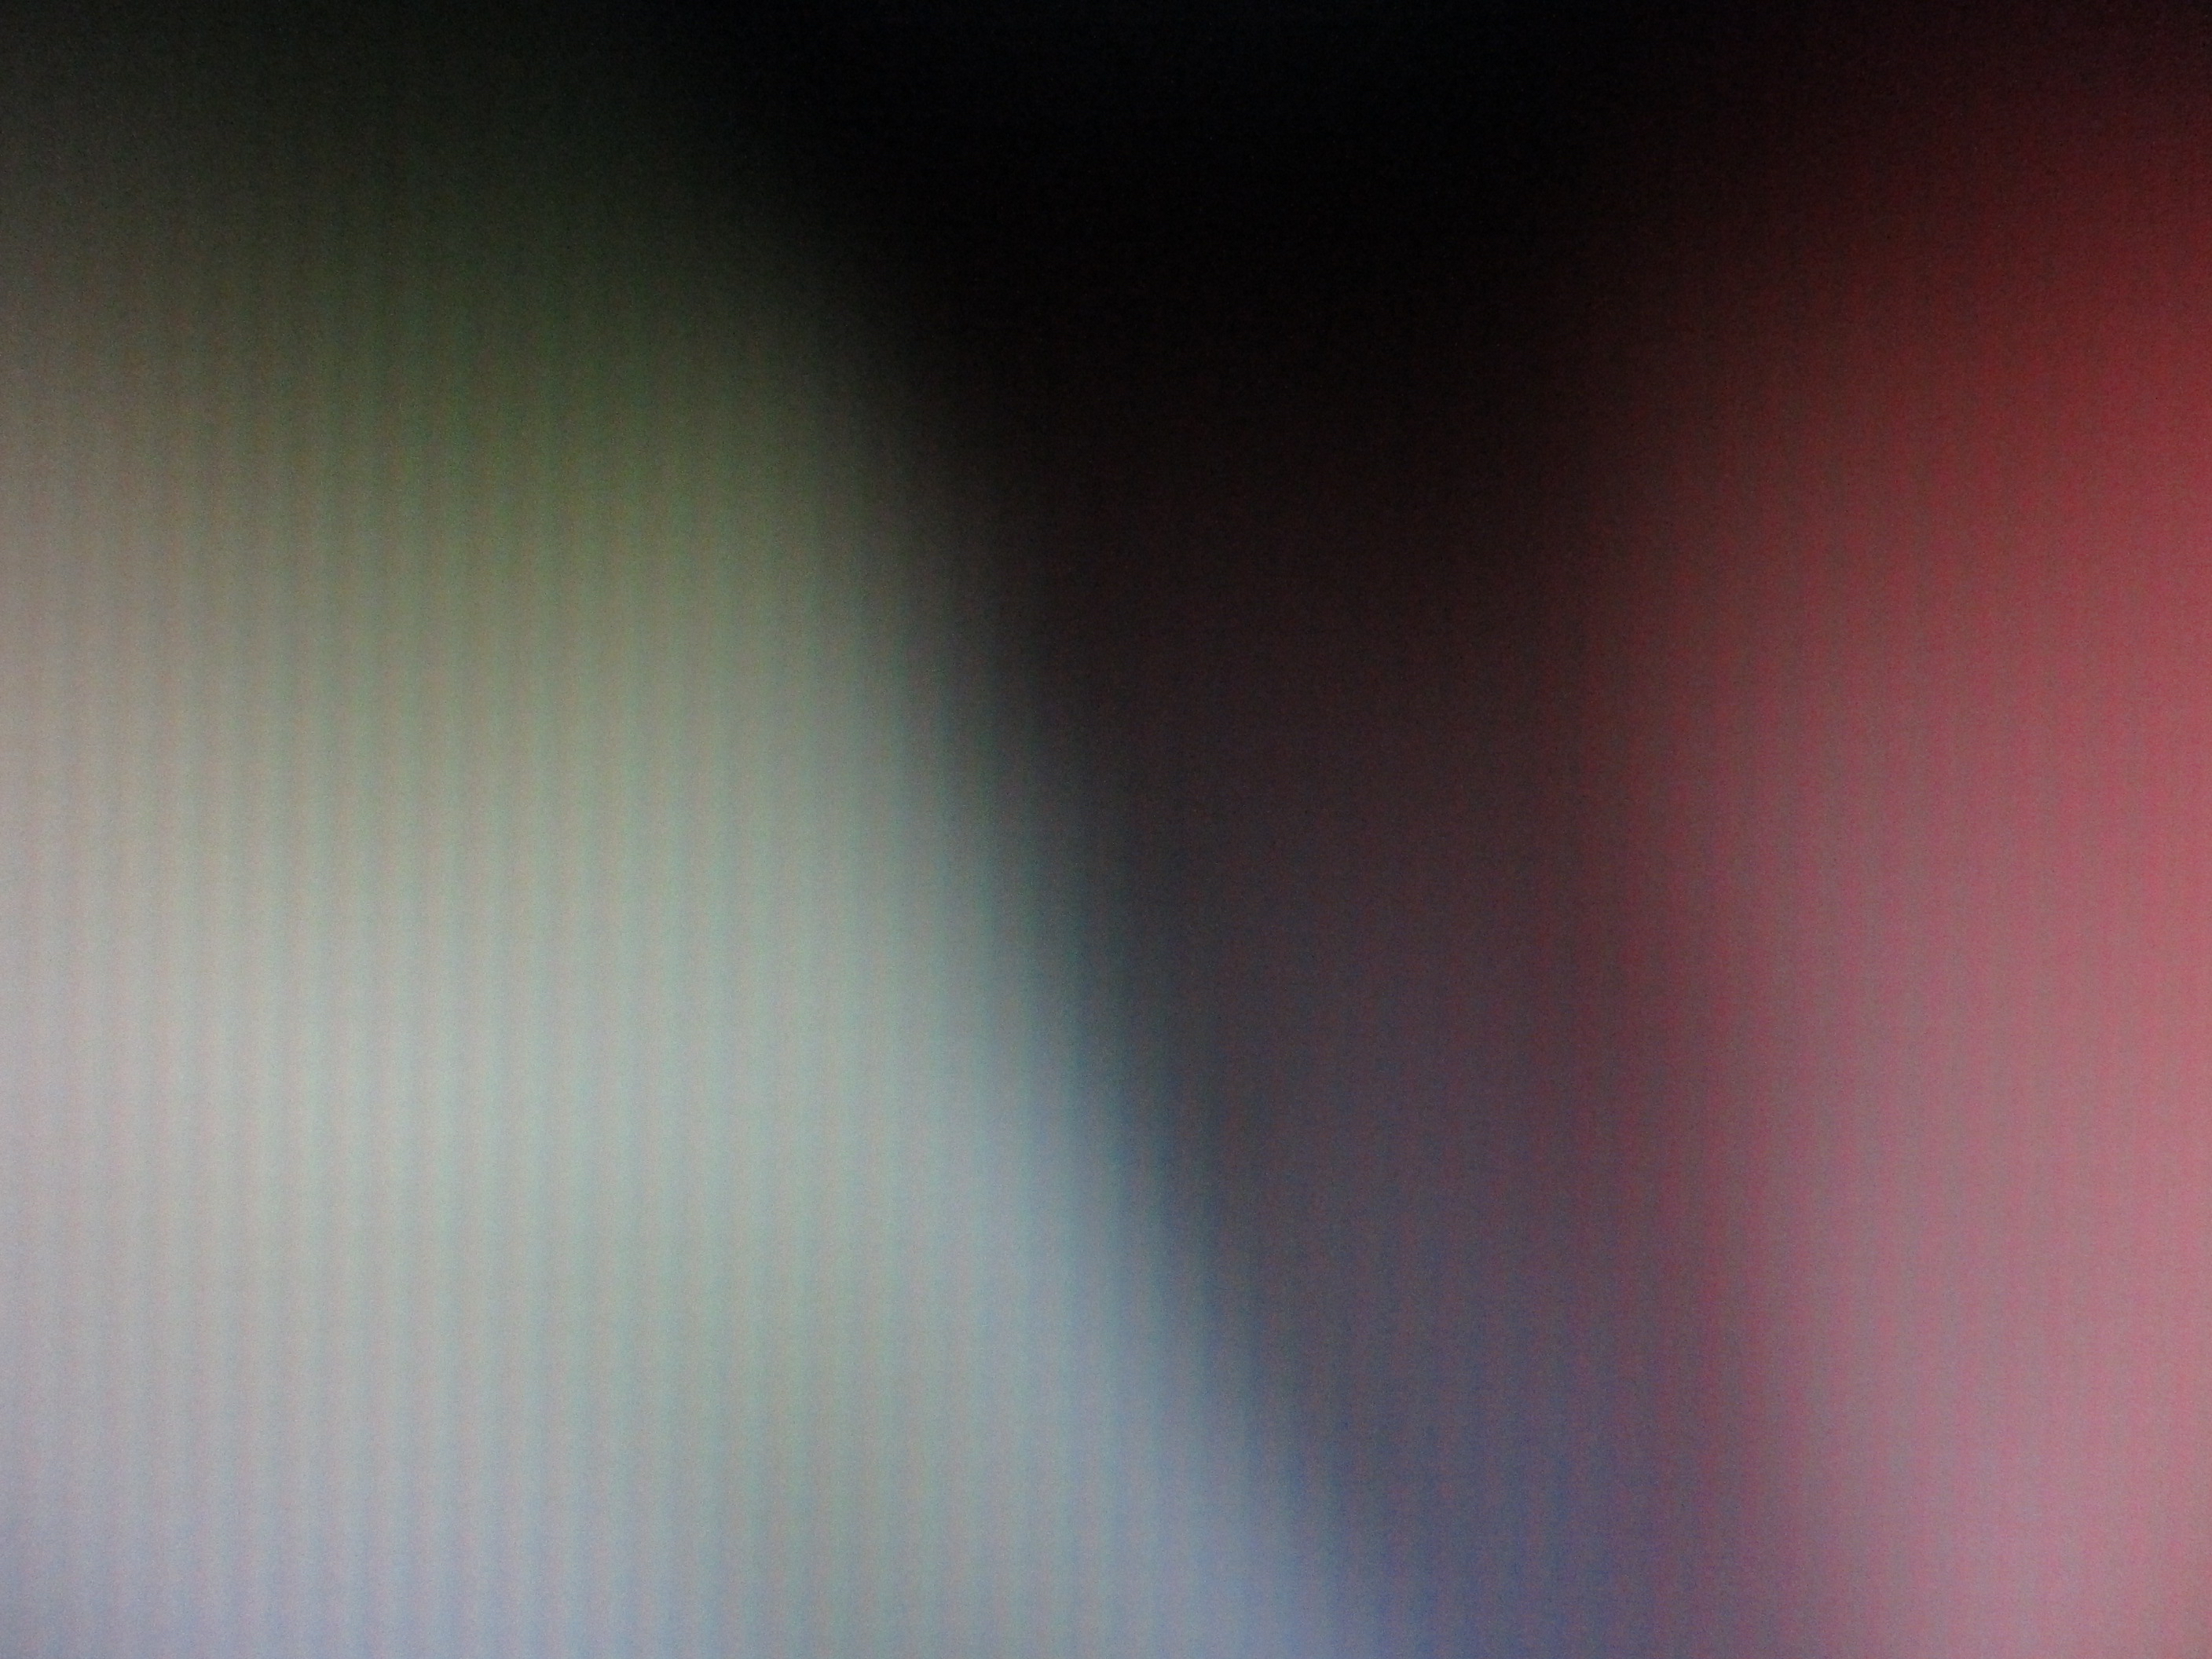
\includegraphics[width=0.50\textwidth]{physiology/tv.jpg}
		
		{\scriptsize Photo en gros plan d'une télévision \\ \phantom{x}}
	\end{center}
}


% ------------- %

\frame{
	\frametitle{Problématique 1 - Représenter des images}
	
	\phantom{Solution technique adoptée : }
	
	\phantom{émission de lumières rouge, verte et bleue \og{}mélangées\fg{}}.

	\medskip
	
	\phantom{De petits émetteurs pour chacune des trois couleurs}.
	
	\begin{center}
		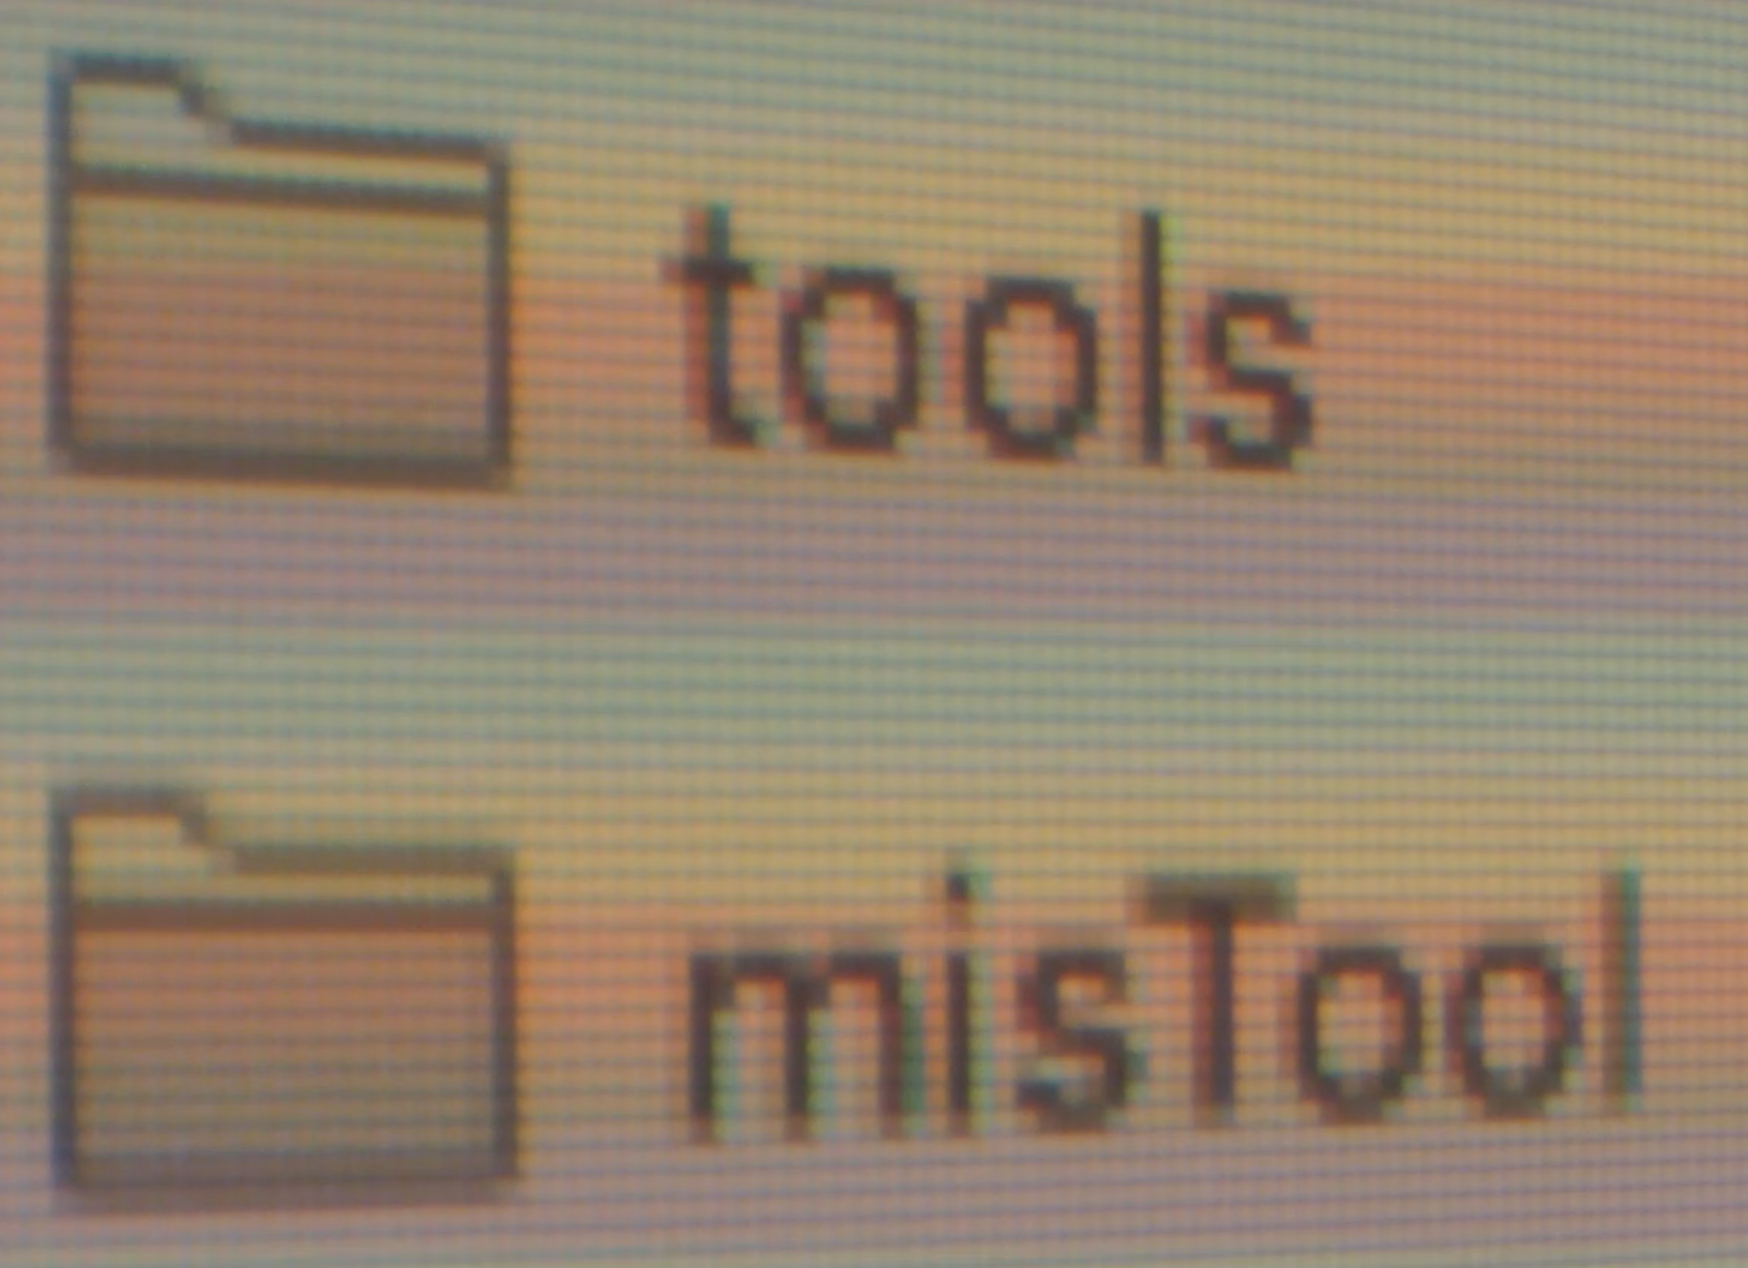
\includegraphics[width=0.50\textwidth]{physiology/videproj.png}
		
		{\scriptsize Image extraite d'une vidéo filmant le rendu d'un vidéo projecteur \\ (le fond était visuellement blanc)}
	\end{center}
}


% ------------- %

\frame{
	\frametitle{Problématique 2 - Capter des images}
	
	Principe \og{}inverse\fg{} de la représentation.
	
	\begin{itemize}[<+(1)->]
		\item Utilisation de petits capteurs spécialisés dans une couleur.
		
		\item Application des résultats de la physique quantique.
		
		\item Mesures électriques traduites en nombres.
	\end{itemize}
}


% ------------- %

\frame{
	\frametitle{Problématique 3 - Coder les images}
	
	\begin{itemize}[<+(1)->]
		\item Comment coder une image ?
		
		\item Quelles conventions utilisées ?
		
		\item Nécessité d'établir des standards.
	\end{itemize}
}


% ------------- %

\begin{frame}[fragile]
	\frametitle{Problématique 4 - Analyser des images}
	
	Problème difficile.
	\pause
	Pourquoi ?
	
	\pause
	
	\medskip 
	
	Imaginons que l'on code par $1$ le noir et $0$ le blanc.
	
	\pause
	
	\medskip 
	
	Seriez-vous me dire ce que représente l'image noir et blanc de dimension 13 \og{}cases\fg{} horizontalement sur 17 verticalement qui est codée ci-dessous ? 
	
	\begin{center}
		\scriptsize
		\begin{verbatim}
00000000000000000001000000000001110000000001010100000001000001000001
00000001000111000001110010111111101001001000100100100100010010010010
00100100100100010010010010001001001001000100100011000001100000111111
10000000000000000
		\end{verbatim}
	\end{center}
\end{frame}


% ------------- %

\begin{frame}[fragile]
	\frametitle{Problématique 4 - Analyser des images}
	
	Réorganisation des chiffres (respect des dimensions).
	
	\begin{center}
		\scriptsize
		\begin{verbatim}
0000000000000
0000001000000
0000011100000
0000101010000
0001000001000
0010000000100
0111000001110
0101111111010
0100100010010
0100100010010
0100100010010
0100100010010
0100100010010
0100100010010
0011000001100
0001111111000
0000000000000
		\end{verbatim}
	\end{center}
\end{frame}


% ------------- %

\frame{
	\frametitle{Problématique 4 - Analyser des images}
	
	Voici l'image (ajout du quadrillage pour les sceptiques).
	
	\begin{center}
		
\includegraphics[scale=0.15]{physiology/crayon.png}
	\end{center}
	
	On devine un crayon...	
	Pas si simple même en noir et blanc !
	
	\pause

	\medskip
	
	Imaginez les problématiques soulevées avec des images en couleur.
}


% ------------- %

\begin{frame}[fragile]
	\frametitle{Problématique 4 - Analyser des images}
	
	\textbf{Attention !} Codons par \verb+#+ le noir et par \verb+.+ le blanc.
	
	\medskip 
	
	On obtient visuellement un crayon.
	
	\begin{center}
		\scriptsize
		\begin{verbatim}
.............
......#......
.....###.....
....#.#.#....
...#.....#...
..#.......#..
.###.....###.
.#.#######.#.
.#..#...#..#.
.#..#...#..#.
.#..#...#..#.
.#..#...#..#.
.#..#...#..#.
.#..#...#..#.
..##.....##..
...#######...
.............
		\end{verbatim}
	\end{center}
\end{frame}


% ------------- %

\frame{
	\frametitle{Problématique 4 - Analyser des images}
	
	Ceci ne signifie pas que ce nouveau codage est meilleur.
	
	\medskip
	
	Pourquoi ?
	\pause
	Tout est dans le \og{}visuellement\fg{}. 
}


% ------------- %


\frame{
	\frametitle{Problématique 4 - Analyser des images}
	
	\begin{center}
		\framebox{\textbf{Ne pas oublier qu'un ordinateur est juste un calculateur !}}
	\end{center} 
}
          

\section{Partie 2 : Numériser les images}  

\subsection{Images numériques}

% ------------- %

\frame{
	\frametitle{Numériser, c'est coder !}

	Quel codage choisir qui réponde aux contraintes technologiques ?
		
	\begin{itemize}[<+(1)->]
		\item Images représentées.
		
		\begin{itemize}[<+(1)->]
			\item Quels émetteurs rouges, verts et bleus activés ?

			\item Quelle intensité pour un émetteur donné ?
		\end{itemize}
		
		\item Images captées.
		
		\begin{itemize}[<+(1)->]
			\item Quantifier les mesures physiques.
		\end{itemize}
			
		\item Nécessité de définir des conventions.
	\end{itemize}
}


% ------------- %

\frame{
	\frametitle{Coder les couleurs}

	Le modèle RVB (Rouge-Vert-Bleu) ou RGB (Red-Green-Blue).
	
	\begin{itemize}[<+(1)->]
		\item Souhait de modéliser les outils physiques utilisés.
		
		\item Pour chaque couleur : valeurs allant de $0$ (intensité nulle) 
		
		à $255$ (intensité maximale).
		
		\item Combien de chiffres nécessaires pour un codage binaire ?
		
		\pause 
		
		$256 = 2^8$ donc besoin d'au moins $3 \times 8 = 24$ 
		chiffres en écriture binaire.
	\end{itemize}
}


% ------------- %

\frame{
	\frametitle{Coder les couleurs}

	Exemples de couleur RGB avec la notation
	(Red , Green , Blue).
	
	\begin{itemize}[<+(1)->]
		\item Quelle couleur correspond à $(255 , 0 , 0)$ ?
		
		\pause
		Avec \LaTeX, on obtient
		\framebox{\textcolor[RGB]{255 , 0 , 0}{$\blacksquare\!\blacksquare\!\blacksquare$}} 
		qui est un rouge.
		
		\item Quelle couleur correspond à $(0 , 255 , 0)$ ?
		
		\pause
		Avec \LaTeX, on obtient
		\framebox{\textcolor[RGB]{0 , 255 , 0}{$\blacksquare\!\blacksquare\!\blacksquare$}} 
		qui est un vert.
		
		\item Quelle couleur correspond à $(0 , 0, 255)$ ?
		
		\pause
		Avec \LaTeX, on obtient
		\framebox{\textcolor[RGB]{0 , 0, 255}{$\blacksquare\!\blacksquare\!\blacksquare$}} 
		qui est un bleu.
		
		\item Quel type de couleur correspond à $(200 , 200, 200)$ ?
		
		\pause
		Avec \LaTeX, on obtient
		\framebox{\textcolor[RGB]{200, 200, 200}{$\blacksquare\!\blacksquare\!\blacksquare$}} 
		qui est un gris.
		
		Plus généralement, $256$ nuances de gris grâce à
		$(n , n , n)$. 
	\end{itemize}
}


% ------------- %

\frame{
	\frametitle{Coder les couleurs}

	Exemples de couleur RGB avec la notation
	(Red , Green , Blue).
	
	\vspace{-.7em}
	\begin{flushright}
		\scriptsize (la suite)
	\end{flushright}
	\vspace{-1.2em}
	
	\begin{itemize}[<+(1)->]		
		\item Comment obtenir du blanc ?
		
		\pause
		$(255 , 255, 255)$ nous donne avec \LaTeX : \framebox{\textcolor[RGB]{255,255,255}{$\blacksquare\!\blacksquare\!\blacksquare$}} .
		
		\item Comment obtenir du noir ?
		
		\pause
		$(0 , 0, 0)$ nous donne avec \LaTeX : \framebox{\textcolor[RGB]{0,0,0}{$\blacksquare\!\blacksquare\!\blacksquare$}} .
		
		\item Proposons un codage correspondant à un jaune.
		
		\pause
		Mélangeons du rouge et du vert (pas simple a priori). 
		
		$(255 , 255, 0)$ nous donne avec \LaTeX : \framebox{\textcolor[RGB]{255,255,0}{$\blacksquare\!\blacksquare\!\blacksquare$}} .
	\end{itemize}
}


% ------------- %

\frame{
	\frametitle{Coder les couleurs}

	Une autre convention pour le format RGB.
	
	\pause
	\medskip
	
	$256 = 2^8 = (2^4)^2 = 16^2$ donc deux chiffres en écriture hexadécimale pour chacune des couleurs.
	
	\pause
	\medskip
	
	Collage successif de ces écritures dans l'ordre R-G-B.
	
	\medskip
	
	$3 \times 2 = 6$ chiffres au total pour les trois couleurs.
	
	\pause
	\medskip
	
	Par exemple, $(0 , 141, 255)$ s'écrit
	\pause
	008DFF ou juste 8DFF
	en utilisant $141 = 128 + 13 = 8 \times 16 + 13$.
	
	\pause
	\medskip
	
	Un autre exemple : (30 , 173, 5) s'écrit
	\pause
	1EAD05.
}


% ------------- %

\frame{
	\frametitle{Repérage des émetteurs et des récepteurs}

	Reste à indiquer où une couleur sera activée, ou bien à savoir 
	
	où elle a été mesurée (quantifiée).
	
	\pause
	\medskip
	
	\textbf{Attention !} Convention des écritures manuscrites  \og{}latines\fg{}
	
	ou de la machine à écrire.
	
	\begin{center}
		\definecolor{qqffqq}{rgb}{0.,1.,0.}
\definecolor{zzttqq}{rgb}{0.6,0.2,0.}
\definecolor{ffqqqq}{rgb}{1.,0.,0.}
\begin{tikzpicture}[line cap=round,line join=round,>=triangle 45,x=0.6cm,y=0.6cm]
\clip(-3.840937894924428,-1.30338099546581) rectangle (6.243481310215926,5.683680882381437);
\fill[color=ffqqqq,fill=ffqqqq,fill opacity=1.0] (0.,4.) -- (1.,4.) -- (1.,3.) -- (0.,3.) -- cycle;
\fill[color=qqffqq,fill=qqffqq,fill opacity=1.0] (2.,2.) -- (3.,2.) -- (3.,1.) -- (2.,1.) -- cycle;
\fill[fill=black,fill opacity=1.0] (-2.,2.) -- (1.,2.) -- (1.,1.) -- (-2.,1.) -- cycle;
\draw (-3.,5.)-- (4.,5.);
\draw (4.,5.)-- (4.,1.);
\draw (4.,1.)-- (-3.,1.);
\draw (-3.,1.)-- (-3.,5.);
\draw (-2.,5.)-- (-2.,1.);
\draw (-1.,1.)-- (-1.,5.);
\draw (0.,5.)-- (0.,1.);
\draw (1.,1.)-- (1.,5.);
\draw (2.,5.)-- (2.,1.);
\draw (3.,1.)-- (3.,5.);
\draw (4.,4.)-- (-3.,4.);
\draw (-3.,3.)-- (4.,3.);
\draw (4.,2.)-- (-3.,2.);
\draw [->] (-3.,5.) -- (-3.,-1.);
\draw [->] (-3.,5.) -- (6.,5.);
\draw (5.681635097358106,5.770118761282641) node[anchor=north west] {$\mathbf{x}$};
\draw (-3.696874763422423,-0.5254400853549817) node[anchor=north west] {$\mathbf{y}$};
\draw [color=zzttqq] (0.,4.)-- (1.,4.);
\draw [color=zzttqq] (1.,4.)-- (1.,3.);
\draw [color=zzttqq] (1.,3.)-- (0.,3.);
\draw [color=zzttqq] (0.,3.)-- (0.,4.);
\draw [color=zzttqq] (2.,2.)-- (3.,2.);
\draw [color=zzttqq] (3.,2.)-- (3.,1.);
\draw [color=zzttqq] (3.,1.)-- (2.,1.);
\draw [color=zzttqq] (2.,1.)-- (2.,2.);
\draw (-2.,2.)-- (1.,2.);
\draw (1.,2.)-- (1.,1.);
\draw (1.,1.)-- (-2.,1.);
\draw (-2.,1.)-- (-2.,2.);
\draw (-2.803683348109992,5.770118761282641) node[anchor=north west] {$\mathbf{0}$};
\draw (-1.7952414275959563,5.770118761282641) node[anchor=north west] {$\mathbf{1}$};
\draw (-0.8012058202321215,5.770118761282641) node[anchor=north west] {$\mathbf{2}$};
\draw (0.19282978713171336,5.770118761282641) node[anchor=north west] {$\mathbf{3}$};
\draw (1.2012717076457486,5.770118761282641) node[anchor=north west] {$\mathbf{4}$};
\draw (2.1953073150095834,5.770118761282641) node[anchor=north west] {$\mathbf{5}$};
\draw (3.203749235523619,5.770118761282641) node[anchor=north west] {$\mathbf{6}$};
\draw (-3.696874763422423,4.948958911721212) node[anchor=north west] {$\mathbf{0}$};
\draw (-3.696874763422423,3.9549233043573766) node[anchor=north west] {$\mathbf{1}$};
\draw (-3.696874763422423,2.946481383843341) node[anchor=north west] {$\mathbf{2}$};
\draw (-3.696874763422423,1.9524457764795058) node[anchor=north west] {$\mathbf{3}$};
\end{tikzpicture}

		
		\vspace{-0.5em}
		{\scriptsize Graphique produit avec GeoGebra}
	\end{center}
}


% ------------- %

\frame{
	\frametitle{Repérage des émetteurs et des récepteurs}
	
	\begin{center}
		\definecolor{qqffqq}{rgb}{0.,1.,0.}
\definecolor{zzttqq}{rgb}{0.6,0.2,0.}
\definecolor{ffqqqq}{rgb}{1.,0.,0.}
\begin{tikzpicture}[line cap=round,line join=round,>=triangle 45,x=0.6cm,y=0.6cm]
\clip(-3.840937894924428,-1.30338099546581) rectangle (6.243481310215926,5.683680882381437);
\fill[color=ffqqqq,fill=ffqqqq,fill opacity=1.0] (0.,4.) -- (1.,4.) -- (1.,3.) -- (0.,3.) -- cycle;
\fill[color=qqffqq,fill=qqffqq,fill opacity=1.0] (2.,2.) -- (3.,2.) -- (3.,1.) -- (2.,1.) -- cycle;
\fill[fill=black,fill opacity=1.0] (-2.,2.) -- (1.,2.) -- (1.,1.) -- (-2.,1.) -- cycle;
\draw (-3.,5.)-- (4.,5.);
\draw (4.,5.)-- (4.,1.);
\draw (4.,1.)-- (-3.,1.);
\draw (-3.,1.)-- (-3.,5.);
\draw (-2.,5.)-- (-2.,1.);
\draw (-1.,1.)-- (-1.,5.);
\draw (0.,5.)-- (0.,1.);
\draw (1.,1.)-- (1.,5.);
\draw (2.,5.)-- (2.,1.);
\draw (3.,1.)-- (3.,5.);
\draw (4.,4.)-- (-3.,4.);
\draw (-3.,3.)-- (4.,3.);
\draw (4.,2.)-- (-3.,2.);
\draw [->] (-3.,5.) -- (-3.,-1.);
\draw [->] (-3.,5.) -- (6.,5.);
\draw (5.681635097358106,5.770118761282641) node[anchor=north west] {$\mathbf{x}$};
\draw (-3.696874763422423,-0.5254400853549817) node[anchor=north west] {$\mathbf{y}$};
\draw [color=zzttqq] (0.,4.)-- (1.,4.);
\draw [color=zzttqq] (1.,4.)-- (1.,3.);
\draw [color=zzttqq] (1.,3.)-- (0.,3.);
\draw [color=zzttqq] (0.,3.)-- (0.,4.);
\draw [color=zzttqq] (2.,2.)-- (3.,2.);
\draw [color=zzttqq] (3.,2.)-- (3.,1.);
\draw [color=zzttqq] (3.,1.)-- (2.,1.);
\draw [color=zzttqq] (2.,1.)-- (2.,2.);
\draw (-2.,2.)-- (1.,2.);
\draw (1.,2.)-- (1.,1.);
\draw (1.,1.)-- (-2.,1.);
\draw (-2.,1.)-- (-2.,2.);
\draw (-2.803683348109992,5.770118761282641) node[anchor=north west] {$\mathbf{0}$};
\draw (-1.7952414275959563,5.770118761282641) node[anchor=north west] {$\mathbf{1}$};
\draw (-0.8012058202321215,5.770118761282641) node[anchor=north west] {$\mathbf{2}$};
\draw (0.19282978713171336,5.770118761282641) node[anchor=north west] {$\mathbf{3}$};
\draw (1.2012717076457486,5.770118761282641) node[anchor=north west] {$\mathbf{4}$};
\draw (2.1953073150095834,5.770118761282641) node[anchor=north west] {$\mathbf{5}$};
\draw (3.203749235523619,5.770118761282641) node[anchor=north west] {$\mathbf{6}$};
\draw (-3.696874763422423,4.948958911721212) node[anchor=north west] {$\mathbf{0}$};
\draw (-3.696874763422423,3.9549233043573766) node[anchor=north west] {$\mathbf{1}$};
\draw (-3.696874763422423,2.946481383843341) node[anchor=north west] {$\mathbf{2}$};
\draw (-3.696874763422423,1.9524457764795058) node[anchor=north west] {$\mathbf{3}$};
\end{tikzpicture}

	\end{center}

	\vspace{-0.5em}
	
	Cellule \textcolor[RGB]{255,0,0}{rouge} en 
	\pause
	$(x , y) = (3, 1)$.
	
	\medskip
	
	Cellule \textcolor[RGB]{0,255,0}{verte} en 
	\pause
	$(x , y) = (5, 3)$.
	
	\medskip
	
	Couleur des cellules en $(1, 3)$ , $(2, 3)$ et $(3, 3)$ :
	\pause
	le noir. 
}

          

\section{Partie 3 : Quelques formats d'images}  

\subsection{Formats classiques d'images}

% ------------- %

\frame{
	\frametitle{Formats \texttt{ASCII}}

	Caractéristiques générales.

	\begin{itemize}[<+(1)->]		
		\item Formats \texttt{ASCII} \og{}manipulables à la main\fg{}.

		\begin{itemize}	
			\item Windows : utilisation de Notepad++.
			
			\item Linux : Geany.
			
			\item Mac OS : Atom.
		\end{itemize}		
		
		\item Formats pris en charge par Gimp.
		
		\item Trois versions.

		\begin{itemize}	
			\item Portable Bitmap (PBM) : image en noir et blanc.
			
			\item Portable Graymap (PGM) : image en niveau de gris.
			
			\item Portable Pixmap (PPM) : image en couleur.
		\end{itemize}
		
		\item Pour ceux présentés, pas de compression : les infos de chaque pixel directement dans le fichier image.
	\end{itemize}		
}


% ------------- %

\frame{
	\frametitle{Formats \texttt{ASCII} : Portable Bitmap (PBM)}

	Spécifications techniques du fichier.

	\begin{itemize}[<+(1)->]		
		\item Extension du fichier : \texttt{.pbm}.
		
		\item 1ère ligne ne contenant que le texte \texttt{P1}.
		
		\item 2ème ligne : dimensions sous la forme 
		\texttt{LARGEUR HAUTEUR}.
		
		\item À partir de la 3ème ligne.

		\begin{itemize}	
			\item \texttt{1} code le noir et \texttt{0} le blanc.
			\item Espaces possibles mais pas indispensables.
			\item Pas plus de 70 caractères par ligne.
		\end{itemize}
		
		\item Des commentaires : texte précédé par le symbole \texttt{\#}.
	\end{itemize}		
}


% ------------- %

\begin{frame}[fragile]
	\frametitle{Formats \texttt{ASCII} : Portable Bitmap (PBM)}

	Un exemple.

	\begin{multicols}{2}
		\scriptsize
		\begin{verbatim}
P1     # Image en noir et blanc
13 11  # Largeur = 13  Hauteur = 11
0000000000000
0000000000000
0001111100000
0001000100000
0001011111000
0001010101000
0001111101000
0000010001000
0000011111000
0000000000000
0000000000000
		\end{verbatim}
		
		\vfill
		\columnbreak
		
		\begin{center}
			\framebox{
\includegraphics[width=0.5\textwidth]{picture/carres.png}}
			
			\medskip
			
			\textbf{ATTENTION !} 
			
			Image encadrée et agrandie.
		\end{center}
	\end{multicols}		
\end{frame}


% ------------- %

\frame{
	\frametitle{Formats \texttt{ASCII} : Portable Graymap (PGM)}

	Spécifications techniques du fichier.

	\begin{itemize}[<+(1)->]		
		\item Extension du fichier : \texttt{.pgm}.
		
		\item 1ère ligne ne contenant que le texte \texttt{P2}.
		
		\item 2ème ligne : dimensions sous la forme 
		\texttt{LARGEUR HAUTEUR}.
		
		\item 3ème ligne : \texttt{MAX} la valeur maximale de niveau de gris.
		
		On doit avoir \texttt{MAX} $\leqslant$ 65 536.
		
		\item À partir de la 4ème ligne.

		\begin{itemize}	
			\item Gris codé de \texttt{0} pour le noir à \texttt{MAX} pour le blanc.
			\item Espaces indispensables.
			\item Pas plus de 70 caractères par ligne.
		\end{itemize}
		
		\item Des commentaires : texte précédé par le symbole \texttt{\#}.
	\end{itemize}		
}


% ------------- %

\begin{frame}[fragile]
	\frametitle{Formats \texttt{ASCII} : Portable Graymap (PGM)}

	Un exemple.

	\begin{multicols}{2}
		\scriptsize
		\begin{verbatim}
P2   # Image en niveau de gris
8 7  # Largeur = 8  Hauteur = 7
10   # 11 Niveaux de gris
10 10 10 10 10 10 10 10
10 0  0  0  0  0  10 10
10 0  10 10 10 0  5  10
10 0  10 10 10 0  5  10
10 0  10 10 10 0  5  10
10 0  0  0  0  0  5  10
10 10 5  5  5  5  5  10
10 10 10 10 10 10 10 10
		\end{verbatim}
		
		\vfill
		\columnbreak
		
		\vspace{-0.5em}
		
		\begin{center}
			\framebox{
\includegraphics[width=0.5\textwidth]{picture/carre_ombre.png}}
			
			\medskip
			
			\textbf{ATTENTION !} 
			
			Image encadrée et agrandie.
		\end{center}
	\end{multicols}		
\end{frame}


% ------------- %

\frame{
	\frametitle{Formats \texttt{ASCII} : Portable Pixmap (PPM)}

	Spécifications techniques du fichier.

	\begin{itemize}[<+(1)->]		
		\item Extension du fichier : \texttt{.ppm}.
		
		\item 1ère ligne ne contenant que le texte \texttt{P3}.
		
		\item 2ème ligne : dimensions sous la forme 
		\texttt{LARGEUR HAUTEUR}.
		
		\item 3ème ligne : \texttt{MAX} la valeur maximale pour le rouge, le vert et le bleu. On doit avoir \texttt{MAX} $\leqslant$ 65 536.
		
		\item À partir de la 4ème ligne.

		\begin{itemize}	
			\item Couleur codé au format R G B.
			\item Espaces indispensables.
			\item Pas plus de 70 caractères par ligne.
		\end{itemize}
		
		\item Des commentaires : texte précédé par le symbole \texttt{\#}.
	\end{itemize}		
}


% ------------- %

\begin{frame}[fragile]
	\frametitle{Formats \texttt{ASCII} : Portable Pixmap (PPM)}

	Un exemple.

	\begin{center}
		\scriptsize
		\begin{verbatim}
P3   # Image en couleur
7 2  # Largeur = 7 Hauteur = 2
10   # 11 niveaux pour R, V ou B
0 0 0   5 0 0   0 0 0   0 5 0   0 0 0   8 8 8   0 0 0
0 0 0   5 0 0   0 0 0   0 5 0   0 0 0   8 8 8   0 0 0
		\end{verbatim}
		
		\bigskip
		
		\framebox{
\includegraphics[width=0.5\textwidth]{picture/trois_traits.png}}
		
		\medskip
			
		\textbf{ATTENTION !} 
			
		Image encadrée et agrandie.
	\end{center}		
\end{frame}


% ------------- %

\frame{
	\frametitle{Formats utiles pour le web}

	\og{}Non manipulables à la main\fg{} :
	utilisation de pillow (Python 3).

	\begin{itemize}[<+(1)->]		
		\item Graphics Interchange Format (GIF)
		
		\begin{itemize}		
			\item Extension du fichier : \texttt{.gif}.
			\item Transparence et compression (avec perte).
			\item Affichage progressif.
		\end{itemize}
	
		\item Portable Network Graphics (PNG) 
		
		\begin{itemize}		
			\item Extension du fichier : \texttt{.png}.
			\item Transparence et compression sans perte.
			\item Affichage progressif.
		\end{itemize}
	
		\item Joint Photographic Experts Group (JPEG)
		
		\begin{itemize}		
			\item Extension du fichier : \texttt{.jpg} ou \texttt{.jpeg}.
			\item Pas de transparence mais compression réglable  (avec perte).
			\item Affichage progressif.
		\end{itemize}
	\end{itemize}		
}



\section{Sources utilisées}  

\begin{frame}
	\frametitle{Références}

	\begin{itemize}
		\item \textit{\og{}Introduction au traitement d'images [2\textup{e} édition]\fg{}} de Dian \textsc{Lingrand} édité par Vuibert.

		\item \textit{\og{}Formation \textsc{\textit{Lyon}} ISN 2015 : Modules \& Représentation d'images\fg{}} de Nicolas-François \textsc{Buyle-Bodin}.

		\item \textit{\og{}Numérisation [Cours ISN 2012-13]\fg{}} de Xavier \textsc{Ouvrard}.
		
		\item \url{fr.wikipedia.org/wiki/Portable_pixmap}
		
		\item \url{fr.wikipedia.org/wiki/Graphics_Interchange_Format}
		
		\item \url{fr.wikipedia.org/wiki/Portable_Network_Graphics}
		
		\item \url{fr.wikipedia.org/wiki/JPEG}
	\end{itemize}
\end{frame}
 
\end{document}
